% 1977 年广西百色卷（文科）第 3 题：圆内接三角形 ABC，AD、BE 分别为 BC、AC 边上的高，
% AD 延长交外接圆于 F，虚线 DF、BF（按源卷第 3 页布局：A 左上、B 左、C 右、F 底部，E 在 AC 上近 A，D 在 BC 上）
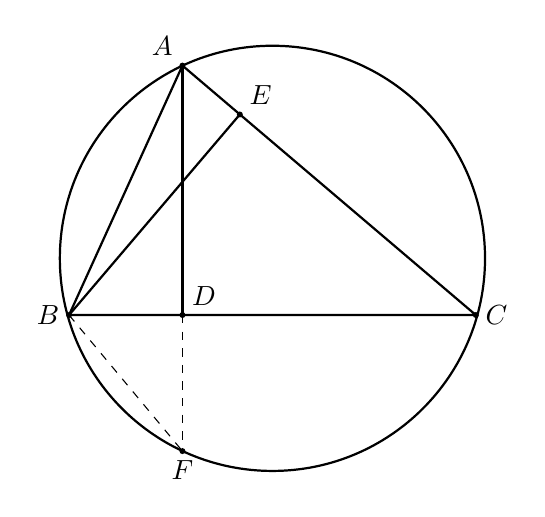
\begin{tikzpicture}[scale=0.9]
  \draw[thick] (0,0) circle (3);
  \coordinate (A) at (-1.27,2.72);
  \coordinate (B) at (-2.87,-0.8);
  \coordinate (C) at (2.87,-0.8);
  \coordinate (D) at (-1.27,-0.8);
  \coordinate (E) at (-0.46,2.03);
  \coordinate (F) at (-1.27,-2.72);
  \draw[thick] (A)--(B)--(C)--cycle;
  \draw[thick] (B)--(E);
  \draw[thick] (A)--(D);
  \draw[dashed] (D)--(F);
  \draw[dashed] (B)--(F);
  \fill (A) circle (1.2pt) node[above left] {$A$};
  \fill (B) circle (1.2pt) node[left] {$B$};
  \fill (C) circle (1.2pt) node[right] {$C$};
  \fill (D) circle (1.2pt) node[above right] {$D$};
  \fill (E) circle (1.2pt) node[above right] {$E$};
  \fill (F) circle (1.2pt) node[below] {$F$};
\end{tikzpicture}
